\documentclass[]{article}
\usepackage{cite}
\usepackage{hyperref}
\usepackage{multicol}
\usepackage{graphicx}
\usepackage{listings}
\usepackage{pgfplots}
\usepackage{tcolorbox}
\usepackage{tikz}
\usepackage{tikz-qtree}

\graphicspath{ {images/} }
\setlength{\parskip}{0.5em}
\pgfplotsset{width=10cm,compat=1.9}

\begin{document}

\begin{titlepage}
    \begin{center}
        \vspace*{1cm}
        
        \Huge
        \textbf{Using WordNet and the Working Memory Model for Semantic Analysis}
        \vspace{2cm}
        
        \Large
        \textbf{William T. F. Strachan}
        
        \vfill
                
        \vspace{0.8cm}
        
        \Large
        Wordcount - 11798\\
        \small
        (Wordcount produced using wc - w, \\
        this includes all the body of the report,\\
         and Appendix A)\\
        \large
        \vspace{0.8cm}
        Supervisor - Dr Dimitar Kazakov\\
        Department of Computer Science\\
        University of York\\
        25 April 2017
        
    \end{center}
\end{titlepage}
\
\vfill
\begin{center} 
	\textbf{Abstract}
\end{center} 
\label{sec:Abstract}
Semantic Analysis is the process of giving meaning to the tokens of a sentence. This process has a multitude of applications from speech recognition to unsepervised knowledge aquisition. Current solutions do not provide enough accuracy to be relied upon fully for these puposes, making it a heated area of research. It is known that humans are very good at semantic analysis, and multiple psychologial models describing this exist, such as the Working Memory Model. The focus of this report is a computational model, derived from these theories, with the intention of providing a more reliable solution to the problem of semantic analysis. A subset of the working memory model is used, in conjunction with hyponymy based activation and disambiguation. The model developed provides an acccuracy greater than some approaches, though, without further development, fails to reliably identify word meanings across a large input corpus. The results implicate the need for the use of a greater number of semantic links in order to correctly derive meaning.

\vfill

\newpage

\tableofcontents
\listoffigures
\listoftables


\newpage
% ------------------------------ START OF DISSERTATION ------------------------------

\section{Introduction}
\label{sec:Intro}
%--------------------- NLP

\subsection{Context}
\label{sec:IntroContext}

Natural language is the language spoken and written by humans. It is very powerful, though its key downfall is its ambiguity. The study of natural language processing (NLP) aims to allow a computer to understand natural language, and formulate a relevant response based upon its input. Within this, the problem of input text analysis has traditionally been broken down into smaller sub-problems \cite{NLPHandbook}:

\begin{itemize}
	\item \textbf{Text Preprocessing} \\
	Before any analysis can take place, the input raw text must be converted into a usable format \cite{NLPHandbook}.
	\item \textbf{Lexical Analysis} \\
	One word can have multiple forms, for example ”judge” (the lemma) has the forms {”judge”, ”judges”, ”judging”, ”judged”} (morphological variants). The job of Lexical Analysis is to replace all morphological variants of a word, with their corresponding lemma, a process known as stemming \cite{NLPHandbook}.
	\item \textbf{Syntactic Parsing} \\
	When deriving meaning from sentences, the grammatical structure can provide important insight. The Syntactic parsing technique extracts this information using Part-of-Speech (PoS) tagging (detecting syntactic role) and Chunking (detecting noun and verb phrases) \cite{NLPHandbook}.
	\item \textbf{Semantic Analysis} \\
	The derivation of meaning from the sentences tokens \cite{NLPHandbook}. 
\end{itemize}

Semantic analysis is a problem which continues to draw attention from researchers, due to the lack of a truly capable solution \cite{NLPHandbook}. If found, a reliable semantic analysis system would have many applications, a subset of these being:

\begin{itemize}
	\item \textbf{Voice Recognition} has, over recent years, become an increasingly useful feature in consumer electronics. Conceptually, it can be seen that a system's ability to respond to voice input would be improved by a better semantic analysis.
	
	\item \textbf{The Summarisation of Documents} is a problem that has been partially solved by \hyperref[sec:TFIDF]{TF-IDF}. The summarisation could be improved by the aquisition of information regarding text meaning.
	 
	\item \textbf{The Aquisition of Information for knowledge based systems} could occur automatically,using an effective semantic analysis system in conjunction with a large corpura.
\end{itemize}

Most would agree that, though a good computational solution is not available, the human brain performs impressively well when confronted with the same problem. Given the example:

\[The\: party\: led\: government\]

it is known by the reader that “party” refers to a political party, due to the fact that it is leading government. The meaning of the word is taken from its surrounding context.

It can be seen that the study of the brain's processes of semantic analysis, and their application to a computational model, could provide a satisfying solution. A great deal of research is directed at studying these processes, largely influenced by the Working Memory model proposed by Baddeley \cite{MemoryBaddeleyEysenkAnderson}. This memory model describes a system of structures, which work in conjunction with one another to form a representation of the brain’s input. 

The Working Memory model has many more applications than the one described in the coming report, requiring more structures than are relevant to the process of semantic analysis. For the purposes of this application, we will restrict our focus to three of these memories, short-term, long-term, and the Episodic buffer\cite{MemoryBaddeleyEysenkAnderson}; each of which is described in greater detail in the Literature review.

\subsection{Problem Definition}
\label{sec:IntroProbDef}

The following report will discuss and define a potential computational model of the psychological theories surrounding the process of Semantic Analysis, with a specific focus on Baddeley's Working Memory Model. As part of the project, a system will be built, and tested against an input corpus. Due to time, and performance constraints, a level of abstraction will be required. It is the purpose of this testing to decide whether the level of abstraction used provides a satisfactory performance.

\subsection{Ethics}
\label{sec:IntroEthics}

The project conducted as part of this report requires no outside participants, nor does it directly contribute to any research or action that could lead to harm. The purposes of this project are purely research based, with the intention of leading to further research in the same field. It is assumed that previous research used by this project was conducted following generally accepted ethical practices.

\section{Literature Review}
\label{sec:LitReview}

In the introduction, the basic motivations behind this project have been established. This literature review aims to describe, and discuss, the previous research, upon which this project is built. The following section will cover Psycholinguistics, previous work on semantic analysis, as well as some of the tools that are used throughout the implementation.

%------------ Memory Models
\subsection{Psycholinguistics}
\label{sec:Psycholinguistics}
The understanding of natural language is a problem with which the human brain performs extremely well. From this statement, it can be derived that a computational solution could be effectively built around knowledge of the processes at work in the brain. The process of language comprehension can be described, in part, using the Working Memory model\cite{MemoryBaddeleyEysenkAnderson}.

According to Baddely et al. \cite{MemoryBaddeleyEysenkAnderson} there exist multiple, special purpose, memory structures within two main categories, the Short-term Memory and the Long-term Memory. The Working Memory model describes how information can pass between the different structures, either originating from the Long-term Memory, or sensory inputs \cite{MemoryBaddeleyEysenkAnderson}.

\subsubsection{Long-term Memory}
\label{LongTerm}
The long-term memory (LTM) contains semi-permanent information. Within the LTM, there exist explicit and implicit memory structures. The contents of the Implicit memory describe skills and methods of doing things, whereas the Explicit memory contains factual information\cite{MemoryBaddeleyEysenkAnderson}. When considering these structures, it can be seen that Explicit memory is of greater interest in the context of NLP.

Within the Explicit memory exists knowledge of semantics \cite{MemoryBaddeleyEysenkAnderson}. The information held here not only defines concepts (meanings of word forms), but also their attributes and rules of use. In 1966, M. Quillain proposed a model of Semantic Memory \cite{SemanticMemoryQuillain}. The model consists of a graph of nodes, each representing a concept, connected by edges of differing types, each representing a different syntactic feature (for example, hypernym).  


\subsubsection{Short-term Memory}
\label{ShortTerm}
The short-term memory (STM) is a structure of finite capacity, used to store items for periods usually of no more than 15-30 seconds \cite{MemoryBaddeleyEysenkAnderson}. In 1956, G. Miller, based upon previous experimental results, concluded that the finite size of the STM existed in the realm of 7$\pm$2 items of information \cite{SevenPlusMinusTwo}. 

In 1971, R. Atkinson and R. Shiffrin proposed a model of the STM \cite{ControlProcessesSTMAtkinson}. In this model, the STM can both send information to, and draw information from the LTM. Inputs from the sensory registers (memory structures holding information relating to inputs from senses) are also sent to the STM. Atkinson and Shiffrin proposed that, over time, the activation of items in the STM decreased; they went on to theorise that items could only be lost from the STM when a new, more highly activated item could take its place. To counter this loss of activation, the authors discussed the control process, rehearsal. This process makes use of repetition to increase the activation of items in memory, decreasing their chance of loss. 

\subsubsection{Episodic Buffer}
\label{sec:EpisodicBuffer}
When considering the reading of text, it was found that participants were able to recall significantly more than 7$\pm$2 items of information. In 2000, a structure linking the STM and LTM was proposed by Baddely \cite{BaddeleyEpisodicBuffer}. The Episodic Buffer acts as a bridge between the LTM and STM, storing information too old to exist in the STM, without committing it to the LTM. This often occurs through the use of imagery to represent a set of concepts \cite{MemoryBaddeleyEysenkAnderson}. When applied to natural language, this memory structure allows the representation of a greater context than the STM alone.

\subsubsection{Disambiguation Models}
\label{sec:DisambiguationModels}
In some cases, when assigning meaning to words, ambiguity can arise. Some words have multiple concepts, for example, bank can refer to a building, or a sloped surface alongside a body of water. In such cases, the brain uses some process to select the correct concept. One such model of this disambiguation is the Multiple-Access model \cite{PsychologyOfLanguage}.

According to the Multiple-Access model, when presented with an ambiguious word, initially all corresponding concepts are activated \cite{AccessingLexicalAmbiguities}. The most appropriate concept is then chosen using a balance of context and frequency.

The context-sensitive model extends the multiple-access model, by more appropriately using context and frequency in the selection of the most appropriate of concept \cite{PsychologyOfLanguage}. In cases where the context is strong, i.e. the correct concept can be chosen using it's surrounding context, the context is primarily relied upon for disambiguation. In the opposite case, i.e. when context gives little indication of which is the correct concept, the most frequently used concept is used, assuming it fits with the available context.


%------------ WORDNET
\subsection{Wordnet}
\label{Wordnet}
In order to build a successful system, within the time bounds given by this project, a good, pre-existing, model of semantic memory is required. One such example of this is Wordnet \cite{WN1Introduction}.

In 1990, it was noted by G. Miller et al. that current attempts to organise the English lexicon, i.e. conventional dictionaries, offered few benefits when used in conjunction with computers \cite{WN1Introduction}. Wordnet was an effort to produce a dictonary, containing more information than a conventional dictionary, that could be useful for computational applications.

\label{Synsets}Central to the design of Wordnet, is the idea of synsets \cite{WN1Introduction}. The authors began using the assumption that all word meanings can be uniquely defined by their set of synonyms (words which share like meaning). In most cases, this assumption holds true, though, in cases where more detail is required, a "gloss", a brief defininition, was added \cite{WN1Introduction}.

Wordnet builds upon models of the semantic memory, such as that discussed in the \hyperref[LongTerm]{Long-term memory section} \cite{WN1Introduction}. The overall structure relies on four main semantic relations:

\begin{itemize}
	\item Synonymy
	\begin{itemize}
		\item If two words are to be called synonyms, they must share at least one like meaning.
	\end{itemize}
	
	\item Antonymy \label{Antonym}
	\begin{itemize}
		\item Conceptually, Antonymy can be seen as the opposite of Synonymy. Antonymy is difficult to define, as not all words which share opposite meaning can be called antonyms, for example, \{up, down\} is an antonym pair, but \{up, fall\} is not.
	\end{itemize}
	
	\item Hyponymy \label{Hypernym}
	\begin{itemize}
		\item If we consider a a synset to be a object-oriented class, its hypernym can be considered its parent class, for example, birch is a type of tree.
	\end{itemize}
	
	\item Meronymy \label{Meronym}
	\begin{itemize}
		\item Meronymy is relationship between two synsets where one is a part of another, for example, a goat has horns, therefore horn is a meronym of goat.
	\end{itemize}
	
\end{itemize}

It is common knowledge that words can fall into one of a number of categories, nouns, adjectives, verbs and adverbs. G. Miller et al. note that, due to the differences in the relations between words in these categories, each type differs in the structure they imply, and are therefore held in different files \cite{WN1Introduction}. The proceeding subsections will go into each of these categories in more detail.

\subsubsection{Nouns}
\label{Nouns}
G. Miller et al. note that a noun can be defined using only its immediate hypernym, and how it differs from the other hyponyms of its immediate hypernym \cite{WN2Nouns}. From this, it can be seen that hyponymy is perhaps the most important relation in the organisation of nouns. For this reason, nouns form a strong hierachical structure in Wordnet.

Wordnet's designers stated the assumption that all nouns can be contained in a single hierachial structure \cite{WN2Nouns}. The issue with having a single word, of which all other words are hyponyms, is that this hypernym is relatively meaningless. It was instead decided to divide all words into 25 separate files, each containing a hierachical tree beginning with one of the following synsets \cite{WN2Nouns}:

\begin{multicols}{2}
\begin{itemize}
	\item[] \{act, action, activity\}
	\item[] \{animal, fauna\}
	\item[] \{artifact\}
	\item[] \{attribute, property\}
	\item[] \{body, corpus\}
	\item[] \{cognition, knowledge\}
	\item[] \{communication\}
	\item[] \{event, happening\}
	\item[] \{feeling, emotion\}
	\item[] \{food\}
	\item[] \{group, collection\}
	\item[] \{location, place\}
	\item[] \{motive\}
	\item[] \{natural object\}
	\item[] \{natural phenomenon\}
	\item[] \{person, human being\}
	\item[] \{plant, flora\}
	\item[] \{possession\}
	\item[] \{process\}
	\item[] \{quantity, amount\}
	\item[] \{relation\}
	\item[] \{shape\}
	\item[] \{state, condition\}
	\item[] \{substance\}
	\item[] \{time\}
\end{itemize}
\end{multicols}

Other than synonymy and hyponymy, nouns have three other important features \cite{WN2Nouns}:
\begin{itemize}
	\item Attributes
	\begin{itemize}
		\item The attributes of a noun consist of adjectives which distinguish it from other hyponyms of its hypernym, for example \{huge, green, fluffy\}.
	\end{itemize}		
	
	\item Parts
	\begin{itemize}
		\item The parts of a noun consist of its meronyms, described \hyperref[Meronym]{previously}.
	\end{itemize}		
	
	\item Functions
	\begin{itemize}
		\item The functions of a noun consist of verbs which are associated with its actions, for example chair has the functions \{sit, rest\}.
	\end{itemize}		
	
\end{itemize}

Currently, all the described relations, excluding functions have been implemented into WordNet. Function words are a proposed feature, though adding this semantic link may prove difficult \cite{WN2Nouns}. Each noun has a potentially huge amount of functions, adding all of these may prove to be redundant, therefore it may be more useful for the most common (i.e. the most useful) to be included.

\subsubsection{Adjectives}
\label{Adjectives}
Adjectives are divisible into four distinct groups, each implying a different structure of semantic links \cite{WN3Adjectives}:
\begin{itemize}
	\item Descriptive Adjectives
	\begin{itemize}
		\item As stated in the \hyperref[Nouns]{previous section}, nouns have attributes. Descriptive adjectives act as modifiers for these attributes: for example, a building has a height, by saying "tall building", the height attribute is given a value \cite{WN3Adjectives}. Antonymy, defined \hyperref[Antonym]{previously}, is considered by wordnet's designers to be the most important relation between descriptive adjectives. Unfortuantely, not all adjectives have antonyms, leading to the designer's addition of an indirect antonym" semantic link, between synonyms of a word and its antonym \cite{WN3Adjectives}. These semantic links give rise to a structure made up of pairs, linked to one another by their synonyms.
	\end{itemize}		
		
	\item Reference-Modifying Adjectives
	\begin{itemize}
		\item Reference-modifying adjectives have an adverb form which can be used to convey the same meaning \cite{WN3Adjectives}. For example, the noun-phrase "the former manager", can be modified to become "the man who was formerly a manager", without diverging from its original meaning. There exist relatively few examples of this category, so no overarching structure emerges, that being said, in some cases, the antonym relation does occur \cite{WN3Adjectives}.
	\end{itemize}
	
	\item Colour Adjectives
	\begin{itemize}
		\item As their name suggests, colour adjectives concern the value of the colour attribute. This definition implies that these words should, in fact, fit into the descriptive adjective category. Their separation is given by colour adjectives lack of true antonym (excluding modifiers such as "light" and "dark") \cite{WN3Adjectives}. The lack of clear semantic relations between these words poses a problem for their organisation, leading wordnet's designers to link them using their definitions, i.e. using hue, lightness and saturation.
	\end{itemize}	
	
	\item Relational Adjectives
	\begin{itemize}
		\item In the phrase "maternal instinct", it can be seen that the adjective is derived from a noun, in this case "mother"; this is the defining feature of relational adjectives \cite{WN3Adjectives}. In wordnet, relational adjectives are linked to their noun form, meaning they do not posess their own structure, instead falling into that described in the \hyperref[Nouns]{Noun section}.
	\end{itemize}		
		
	
\end{itemize}


\subsubsection{Verbs}
\label{Verbs}
In C. Fellbaums 1990 paper, "English Verbs as a Semantic Net", she discussed the lack of true synonymy across the verb category \cite{WN4Verbs}. This is an issue for Wordnet's designers, with their reliance on \hyperref[Synsets]{synsets}. The author goes on to describe the solution, periphrases, the use of verb phrases to give more meaning to a simple verb. In the paper, the example synset, \{swim, travel through water\} was given\cite{WN4Verbs}. 

The relationships between verbs follow a hierachy shown in Figure \ref{fig:WN4Verbs_pp15}, with each type elaborated upon in the following paragraphs.

\begin{figure}[h]
	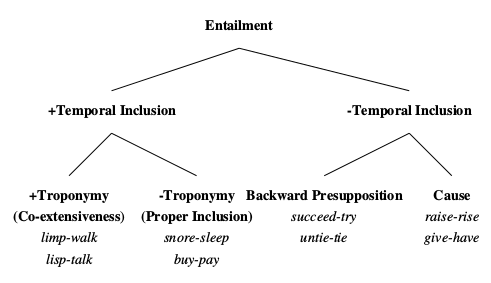
\includegraphics[scale=0.7]{WN4Verbs_pp15.png}
	\caption{HIERACHY OF SEMANTIC RELATIONS BETWEEN VERBS \cite[p.~15]{WN4Verbs}}
	\label{fig:WN4Verbs_pp15}
\end{figure}

\textbf{Entailment} is a relation, simlar in nature to hyponymy. A verb (a) is said to entail another (b) if, when b is substituted for a in a sentence, the truth value of the sentence remains the same \cite{WN4Verbs}. For example, "run" entails "move", "she ran" can also be described by "she moved". If a entails b, and b entails a, a and b are synonyms.

\textbf{Temporal Inclusion} is a form of entailment where one verb (a) is temporally included in another (b) if, b can only occur during the same time period as a\cite{WN4Verbs}. For example, "swallow" is temporally included by "consume". If a can also occur without b, the entailment can be called \textbf{Proper Inclusion}.

\textbf{Troponomy} is a type of entailment where a verb (a) can be said to be a way of doing another verb (b) \cite{WN4Verbs}. For example, "to nap" is a troponym of "to sleep". 

\textbf{Backward Presupposition} is a relation which occurs when one verb (a)  is a precondition of a verb (b) \cite{WN4Verbs}. For example, one must "play" before they can "win".

\textbf{Cause} is a relation where one verb (a) is considered the causative verb, and another (b) is considered the resultative verb, i.e. a causes b to occur \cite{WN4Verbs}. For example, "to teach" is related to "to learn".

The entailment relation leads to a similar structure to that of nouns, a hierachical tree. This structure differs though in its relative lack of depth, caused by the increased average number of concepts per word, when compared to nouns \cite{WN4Verbs}. 

%------------ PREVIOUS WORK
\subsection{Previous Work}
\label{sec:PrevWork}

\subsubsection{Latent Semantic Analysis}
\label{sec:LSA}
In 1997, T. Laundaur and S. Dumais proposed a purely statistical method of semantic analysis, called Latent Semantic Analysis (LSA) \cite{LatentSemanticAnalysis}. The model can be visualised as a set of nodes, each representing a word, existing in semantic space. Words placed close together can be said to have similar meaning, and when close enough together, can be called synonyms. 

When training the model, words which exist in the same context (i.e sentence, paragraph) are linked by a distance derived from their distance in the text. This distance is then adjsted according to similar occurences in more training data. Given enough training data, the distances between each node can be used to give the most likely synonyms of a word, given the context \cite{LatentSemanticAnalysis}.

The authors found that, when presented with a synonym test, the model's best performance gave 64.4\% correct answers , which, when compared to US undergraduates for whom English is not their first language (scoring 64.5\% on average), could be considered to be reasonably effective \cite{LatentSemanticAnalysis}. This model only considers frequency, which, as discussed in the \hyperref[sec:DisambiguationModels]{Disambiguation Models section}, is only one of the two methods the brain is theorised to use for this process. By using a similar method in conjunction with a context focused model, a more accurate and useful model could be produced.

\subsubsection{Extended TF-IDF}
\label{sec:TFIDF}

TF-IDF is an algorithm which, when given a document, outputs its most important words, often used to organise a set of documents into categories. This is done by calculating the importance of each word in the document \cite{TFIDF}, using the formula:
\[t_i = f_t * (log_2(n)-log_2(f_d)+1)\]
Where \(t_i\) is the importance of the word, \(f_t\) is the frequency of the word within the document, \(n\) is the number of documents in the corpura, and \(f_d\) is the frequency of the word across all documents in the corpura \cite{SeddingKazakov}. The  words with the highest importance are then outputted.

In 2004, J. Sedding and D. Kazakov proposed an extension to the TF-IDF algorithm, using \hyperref[Wordnet]{Wordnet}. The aim of the paper was to include extra information provided by Wordnet (synsets and hypernyms) in conjuncton with \hyperref[sec:IntroContext]{PoS tagging} to the existing process. 

As words in a document were encountered, all of its synsets were activated. All hypernyms, to a specified depth were also activated. The output of the system was the set of the most commonly seen synsets across the entire document, according to an equation similar to that discussed earlier in this subsection \cite{SeddingKazakov}.

The authors ran multiple experiments, in order to compare different usage of additional information. Unfortunately, it was found that their method was less effective than TF-IDF alone. As the authors stated, this is likely due to the lack of disambiguation, i.e. all synsets were used for each word, adding noise.

\subsubsection{Neural Networks}
\label{sec:NeuralNetwork}
In recent years the use of Neural Networks, more specifically deep learning Neural Networks, in the solving of computational problems has dramatically increased. More recently, this technique has been applied to the problem of natural language processing. From the description of Natural Language Processing given in the \hyperref[sec:IntroContext]{introduction}, we can see that a large proportion of NLP is the assigning of labels to tokens within a sentence. This process of labelling may also be interpreted as a categorisation problem, which Neural Networks are well suited to, and are often associated with \cite{NeuralNetworks}. 

The first process requrired in the use of neural networks, is the conversion of raw text into a numeric, vector-based representation, capable of being processed. The sentence is then passed into the neural network \cite{NeuralNetworks}. The network proposed by R.Collobert and J. Weston in 2008 contained multiple layers, each serving its own purpose \cite{NeuralNetworks}. Initially the network identifies word features, before using this data to calculate the probability of each synset of each word.

It was found by the authors that their model was capable of producing useful results, though, in order to produce this level of success, a large training dataset was required\cite{NeuralNetworks}. Given the timescale of this project, a neural network based solution, though applicable to psychological theory, would likely be inappropriate.
\subsubsection{Previous use of Wordnet and Short-term Memory for Disabiguation}
\label{sec:MattBurke}

In 2007, a University of York student, M. Burke, produced a project with a simlar aim to the one this report describes. This project builds upon the work and findings of my predecessor. The model developed made use of memory structures based upon those discussed in the \hyperref[sec:Psycholinguistics]{Psycholinguistics section}, i.e. Short-term (STM) and Semantic memories \cite{MattBurkePrevious}. The Short-term memory, was a list, containing synsets, each with its own activation, and Wordnet was used as the Semantic memory, once again each synset has its own activation.    

As words are encountered, their activation, and the activation of their hypernyms is increased. The activation increase of the initial synset was found through experimentation, though the activation increase of hypernyms differed according to the below equation \cite{MattBurkePrevious}. 
\[H = \sum\limits_{i=1}^N S_i \times A\]
Where \(A\) is the attenuation, found through experimentation, \(S_i\) is the activation of the hyponyms. This model was used to prevent more general synsets dominating the short-term memory, whilst boosting hypernyms of synsets more if a similar synset also occurs in close proximity \cite{MattBurkePrevious}.

The author noted that, highly activated synsets could remain in the short-term memory indefinitely. To counter this issue, and to remain in line with the memory models discussed in the \hyperref[ShortTerm]{Short-term memory section}, the process of forgetting was added to the model, by multiplying the activation value by a number found by experimentation \cite{MattBurkePrevious}. Forgetting occurs over time, decreasing the activations of items in the Short-term memory and the Semantic memory, the latter by a greater degree.

In the proposed model, the corpus is processed sentence by sentence. Two methods of disambiguation were proposed, with both cases beginning by removing non-useful words, and converting all words into their base forms (for example, "flies" $\Rightarrow$ "fly"), each model differs in its use of the contents of the short term memory.
\begin{itemize}
	\item[] \textbf{Hypernym-first - } The hypernyms of all words are activated, with the synsets with the highest activation bieng used to disambguate each word \cite{MattBurkePrevious}.
	\item[] \textbf{STM-first - } The contents of the Short term memory's hyponyms are searched until one of the synsets present in the sentence are found \cite{MattBurkePrevious}.
\end{itemize}


As mentioned previously, the values of some variables were found using experimentation. In these experiments, four variables were altered \cite{MattBurkePrevious}:
\begin{itemize}
	\item Disambiguation Method
	\begin{itemize}
		\item[] The author found that STM-first was marginally better (1\% difference)
	\end{itemize}
	\item Short-term memory size
	\begin{itemize}
		\item[] It was found that a STM size of 5 was optimal.
	\end{itemize}
	\item The Attenuation value
	\begin{itemize}
		\item[] The author found that an attenuation value of between 0.7 and 0.9 gave the best result.
	\end{itemize}
	\item Forgetfulness
	\begin{itemize}
		\item[] It was found that a small amount of forgetfulness (multiply activation by 0.95) in conjunction with a small difference in forgetfulness between Semantic and Short-term memories (multiplied by 1.05), produced the best result \cite{MattBurkePrevious}.
	\end{itemize}
\end{itemize}

Unfortunately, the model failed to produce the correct synset significantly more accurately than the author's baseline (selecting the most common synset) \cite{MattBurkePrevious}. As suggested in the report, this may be due to semantic links, which occur in the brain, not being available or utilised by the model. Though, it may also be the case that the mathematical models used were inaccurate, with less linear functions being required.

The memory structures use may also have contributed to the result. Each item in the LTM had an activation \cite{MattBurkePrevious}. This activation is not present in the models developed by either Baddeley, or Shiffrin and Atkinson \cite{MemoryBaddeleyEysenkAnderson, ControlProcessesSTMAtkinson}.

\subsection{SemCor}
\label{sec:SEMCOR}
In order to test the system developed in this project, an input corpus is required. SemCor (semantically-tagged corpus) is a corpus derived from the Brown corpus, containing 352 files \cite{SEMCOR}. The corpus itself has a number of useful features which lend themselves well to this project.

\begin{itemize}
	\item \textbf{Range of Topics} \\
	SemCor is a subset of the Brown corpus, taking documents from the large range of categories available \cite{SEMCOR}. The result is a varied corpus, covering a large range of writing styles. Different styles are likely to make use of words in different manners, providing a more representative view of general performance than a smaller collection of documents.
	
	\item \textbf{PoS Tags} \\
	The corpus has already been syntactically parsed, meaning PoS tags already exist for all words in the corpus \cite{SEMCOR}. This allows the focus of the project to remain on semantic analysis, without the need to build extra sub-systems for preprocessing.
	
		\item \textbf{Ease of Reading} \\
	A reader for SemCor has already been implemented as part of the Natural Language Toolkit for python (NLTK) \cite{NLTK}. The ease of reading provided by NLTK further reduces the scale of the implementation.
	
	\item \textbf{Semantic tags} \\
	The most useful feature of SemCor are the semantic tags. Each tag has been manually added to give the definition of its word. The utilisation of these provide a means for testing the accuracy of the system, by comparing its output to these tags. Each of these tags is a WordNet synset, the same format used as the output of the system, easing comparison \cite{SEMCOR}.
\end{itemize}

\section{Problem Analysis}
\label{sec:ProbAnalysis}

The literature review has given a great deal of indication to the direction of the problem. Given these findings, the problem can be defined with a greater deal of precision. The following can be read as a description of how the implementation should be approached, as well as acting as a set of aims, against which the project will be evaluable.

The overall aim of this project is to build a system capable of finding the correct meaning for each word in an input corpus. Earlier, we established that the brain can reliably solve this problem and, though researchers are currently working to find a suitable computational solution, there exist successful psychological models concerning this process. This project should make use of these psychological models, applying them to a computer system for semantic analysis.

Given the problem described above, and the content of the literature review, we can define three sub-problems. Each of these, when solved individually, should combine to produce a system capable of semantic analysis.

\subsection{Memory Structures}
\label{sec:PAMem}

The brain’s ability to conduct semantic analysis is reliant upon the presence of multiple special purpose memory structures, as described by the Working Memory Model. The most prominent of these are the short-term and long-term memories, both of which should be implemented by an effective system. As part of the working memory model used by this system, information must pass between the each of these memory structures. 

An implementation of the STM should have a finite size, falling in the range defined by G. Miller, 7$\pm$2.  Atkinson and Shiffrin’s model requires that the implemented STM contains items originating from a combination of the systems input, and LTM, each with an activation. The structure’s contents must also change, according to the arrival of new items, so as to correctly represent the local context of a section of text.

The system's LTM (Semantic Memory) requires knowledge of a large number of word meanings. Each of the meanings should be coupled with useful information consisting of a number of semantic links, connecting them to other meanings. As discussed in section \ref{Wordnet}, WordNet is a capable, pre-existing database, which follows a similar structure to the LTM defined by Baddeley. For this reason, it should be used to ensure that as much semantic information can be contained in the LTM as possible within the time scale of the project.

The addition of an Episodic Buffer may also be beneficial. Baddeley’s proposal may prove difficult to implement fully within the scope of this project, so design decisions must be made to simplify the model. With that said, its functionality must remain reasonably consistent, that is, the representation of wider context, for it to prove useful to the system.

\subsection{Reading System}
\label{sec:PARead}

In order for the system to effectively use the memory structures, a reading subsystem is required. In section \ref{sec:SEMCOR}, the input corpus, SemCor, was described. The reading system must be able to accept  this corpus, and feed it into the memory structures described previously. With the focus of this project being solely on semantic analysis, a reading system must also be able to read, and use all relevant information already existing in the input corpus (for example, PoS tags).

In the multiple access model, all relevant concepts are activated when a word is encountered.  A successful reading system should change the contents of the STM using a series of activations. If a concept already exists in the STM, Atkinson and Shiffrin’s model’s process of rehearsal should be employed, increasing the concept's activiation.  

To ensure a good representation of local context in the STM, its contents should consist of relatively general concepts.  For this to occur, activation should make use of hyponomy. M. Burke’s findings on hypernym activation imply that a model will need to be developed, in order to decrease the activations as the hypernym tree is traversed.

\subsection{Disambiguation System}
\label{sec:PADisambiguate}

The multiple access model, and, by extension, the context-sensitive model, requires the usage of both context and frequency to disambiguate tokens.  A system for both methods will need to be developed to ensure that word meanings can be found, regardless of strength of context. There must exist some method of deciding when contextual disambiguation is appropriate, and frequency based methods are not (and vice versa).

A contextual based system must make use of the context held within the system by accessing the contents of the STM.  M. Burke found using a hyponymy to detect similarity between concepts to be reasonably effective. By using at least this semantic relation, a successful system will be able to select from a number of meanings, given the local context alone.

In cases where context is weak, the context-sensitive model tells us that word frequency is used. Given a word, there must exist some method of finding which of its meanings is most likely. 

\subsection{Organisiation}
\label{PAOrganisation}
The project will be conducted roughly in order of the aims discussed previously. The progression of the implementation will occur in an order which allows each section of the system to be tested prior to moving on to the next.

The implementation will take place between week 1 and 8 of term 2. This provides ample time to both implement the system, and evaluate afterwards. In figure \ref{fig:gantt}, a gantt chart specifying an alloted time for each task is given. It is my intention to follow this plan throughout the course of the implementation.

\begin{figure}[h]
	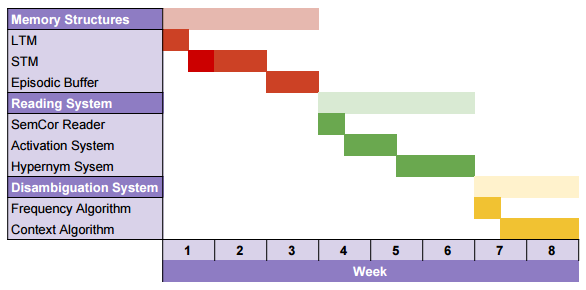
\includegraphics[scale=0.5]{gantt.png}
	\caption{GANTT CHART SHOWING PLAN FOR IMPLEMENTATION}
	\label{fig:gantt}
\end{figure}

Documenting (i.e. the writing of the \hyperref[sec:Implementation]{Design and Implementation} section), as well as testing, is expected to be conducted alongside the implementation process. This will ensure accurate depiction of the design decisions made in the the finalised report.


\section{Design and Implementation}
\label{sec:Implementation}
Given the findings of the literature review, and the definition of the problem given previously, an implementation can be designed. The following section describes the system implemented throughout this project, using pseudocode and diagrams to illustrate. The structure of the section roughly follows the processes conducted by the application, in order, when presented with an input corpus.

The application was implemented using the Python programming language, chosen for the availability of the Natural Language Toolkit (NLTK). NLTK provides an interface for use with Wordnet and a number of useful corpura, specifially SemCor, to be used as test data \cite{NLTK}. All pseudocode given in the following section has been implemented using this language, following the same structure and processes.

\subsection{System Input}
\label{sec:CorpusAnalysis}
The input of the system is a preprocessed document, structured as a series of of hierachical lists \cite{NLTK}:

\begin{itemize}
	\item \textbf{Document}, is a list of paragraphs.
	\item \textbf{Paragraphs}, each of which is a list of sentences.
	\item \textbf{Sentences}, each of which is a list of words.
\end{itemize}

Before a document can be inputted, it must have been syntactically analysed. Each word in a correctly preprocessed document will have a PoS tag, signifying its purpose in the sentence. This tag can then be used to minimise the size of the set of each word's possible definitions.

\subsection{System Output}
\label{sec:SysOutput}
Given an input in the form described \hyperref[sec:CorpusAnalysis]{previously}, after processing, the system will output a document tagged using WordNet synsets. Each synset in the output represents the individual meanings of each word in the document. 

The system currently only considers nouns and verbs, meaning that the output contains no indication of adjective and adverb meanings. Words which do not exist in Wordnet, for example, proper nouns, have also been omitted, as the system is unable to process these.

\subsection{Synsets}
\label{sec:ImplementedSynsets}
In Section \ref{Wordnet}, Wordnet's synsets were described. These synsets are a method of uniquely identifying the meanings of a word, using corresponding synonyms \cite{WN1Introduction}. These synsets are linked to one another by semantic links, accessible through NLTK's Wordnet interface. 

Throughout this implementation, synsets will be used to represent word meanings in both the memory structures and output. This decision has been made due to both their integration with Wordnet, and the effectiveness in which they encode word meaning. 

\subsection{Activation}
\label{sec:activation} 

The corpus is read a sentence at a time, for each word in the sentence a series of activations takes place. Initially, the synsets of each word are activated, followed by their hypernyms following the algorithm outlined in Listing \ref{lst:HypernymActivation}.

\begin{lstlisting}[numbers=left, numberstyle=\small, caption={Hypernym Activation}, captionpos=b, label={lst:HypernymActivation}]
FUNCTION activateHypernyms(synset, depth):
   activationModifier = hypernymModel(depth)
   IF activationModifier < 0 THEN
       RETURN
   ELSE
       FOR hypernym in synset.hypernyms() LOOP
           activateHypernyms(hypernym, depth + 1)
       END LOOP
       RETURN
   END IF
END FUNCTION
\end{lstlisting}

The function recursively traverses the tree of hypernyms, an example of which is shown in Figure \ref{fig:hypernymTree}, activating each synset until, the model gives a result of less than zero. As the function traverses through each hypernym, the amount they are activated by decreases, favouring less general synsets.

\begin{figure}[h]
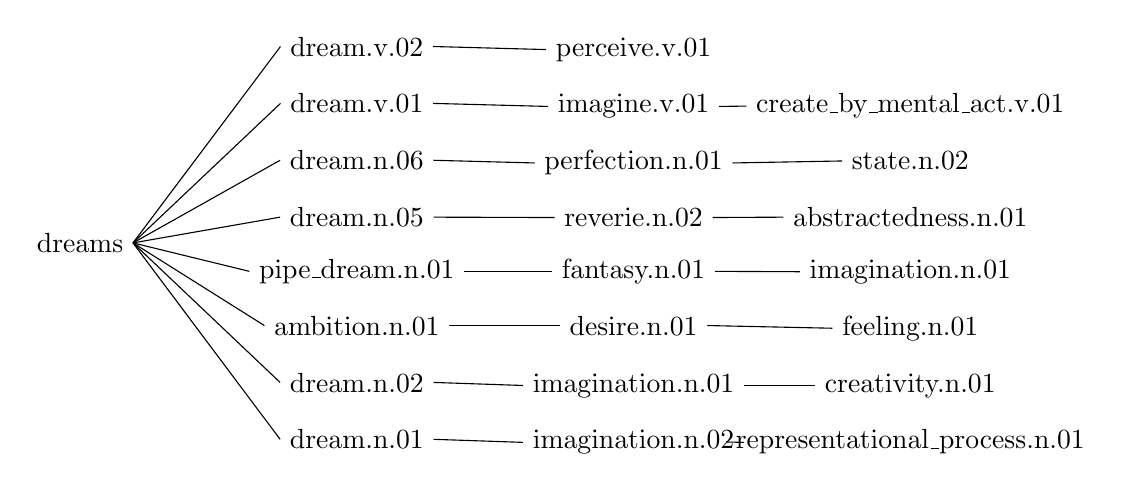
\begin{tikzpicture}[grow=right, sibling distance=5pt, level distance=100pt]
\Tree [.dreams [.dream.n.01 [.imagination.n.02 representational{\_}process.n.01 ] ] [.dream.n.02 [.imagination.n.01 creativity.n.01 ] ] [.ambition.n.01 [.desire.n.01 feeling.n.01 ] ] [.pipe{\_}dream.n.01 [.fantasy.n.01 imagination.n.01 ] ] [.dream.n.05 [.reverie.n.02 abstractedness.n.01 ] ] [.dream.n.06 [.perfection.n.01 state.n.02 ] ] [.dream.v.01 [.imagine.v.01 create{\_}by{\_}mental{\_}act.v.01 ] ] [.dream.v.02 [.perceive.v.01 ] ] ]
\end{tikzpicture}
\caption{HYPERNYM TREE OF "DREAMS"}
\label{fig:hypernymTree}
\end{figure}

\begin{figure}[h]
	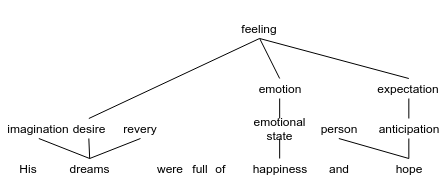
\includegraphics[scale=0.6]{HypernymActivation.png}
	\caption{HYPERNYM ACTIVATION}
	\label{fig:HypernymAct}
\end{figure}

Upon activation, the synset in question's activation is increased by an amount, dependant upon the hypernym model used (discussed later in this section). The same synset can be activated multiple times within the same sentence, an example of which is shown in Figure \ref{fig:HypernymAct}. In this case, a similar model to \hyperref[sec:MattBurke]{that proposed by M. Burke} \cite{MattBurkePrevious} is used: 
\[H = \sum\limits_{i=1}^N S_i\] 
The total activation increase of a synset is equal to the sum of all its activations within the sentence. 

It can be seen that, in Listing \ref{lst:HypernymActivation},  there exists a function, hypernymModel. This function must fit a number of criteria, in order to prevent more general, and therefore less contextually relevant, synsets from dominating the STM.

\begin{itemize}
	\item The activation increase of the word's hypernyms must decrease as their generality increases, i.e.  as they become closer to the top of the tree.
	
	\item Less general hypernyms, i.e. those activated by the first few recursions of activateHypernyms, must be favoured heavily when compared to their more general counterparts.
	
	\item The function must have some method of defining maximum hypernym depth, to prevent the entire tree being activated.
\end{itemize} 

\begin{figure}[h]
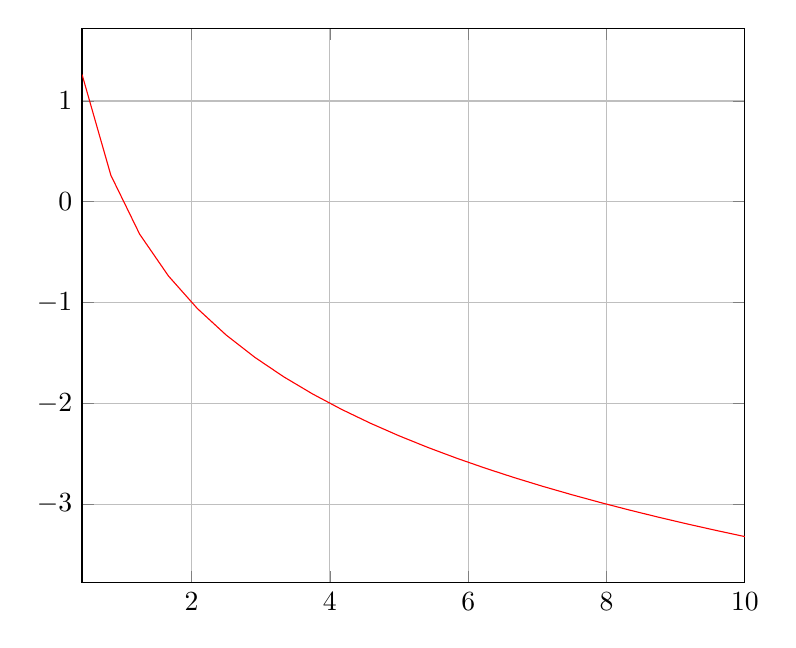
\begin{tikzpicture}
\begin{axis}[domain=0:10, grid=both, enlarge x limits=false]
\addplot[color=red]{-log2(x)};
\end{axis}
\end{tikzpicture}
\caption{GRAPH OF $-\log(x)$}
\label{fig:logGraph}
\end{figure}

One function which fits this criteria is $-\log(x)$, shown in Figure \ref{fig:logGraph}. The values given by the function, for higher values of $x$ are relatively high, favouring more general hypernyms heavily. For lower values of $x$, the values given are relatively low, causing more general hypernyms to have a lower activation increase.

It may be necessary to tune this function during experimentation, to provide greater accuracy, meaning more variables must be added. With these additions, the full model is:
\[f(x) = -b\log(\frac{x}{a})\]
where $a$ and $b$ are varied during experimentation, and $x$ is the depth of the hypernym. $a$ defines where the function passes through the x axis, i.e the maximum hypernym depth, and $b$ defines how steep the function is.

When the depth = 0 (i.e. the activation of the root synset) the model would require the calculation of log(0), which is undefined. For this reason, an offset was added, with a value of 0.001 being used to reduce its impact on the output of the function, making the final model:
\[f(x) = -b\log(\frac{x}{a}+0.001)\]


\subsection{Memory Structures}
\label{sec:ImplementedMemoryStructures}

Upon activation, the synset in question may enter the memory structures, if it posesses a high enough activation. Both an STM and Episodic Buffer have been implemented, using python classes for each. Interactions between the two memory structures are handled by a Memory Controller. 

\subsubsection{STM}
\label{sec:ImplementedSTM}

The STM (Stm in pseudocode) can, in a simplified sense, be described as a list, of finite length, containing memory items. In a more conceptual sense, the STM has been implemented in order to represent the local context of the sentence being analysed, with each synsets relevance being indicated by its activation. 

These memory items held in the STM have been implemented in python as an object with two attributes, synset (immutable), and activation (mutable), based upon the contents of the STM in the working memory model \cite{MemoryBaddeleyEysenkAnderson}. These memory items can be replaced, if a synset with greater activation appears. The process of synset replacement is handled by the swapLowestItem function shown in Listing \ref{lst:swapLowestItem}.

\begin{lstlisting}[numbers=left, numberstyle=\small, caption={the swapLowestItem function}, captionpos=b, label={lst:swapLowestItem}]
FUNCTION swapLowestItem(newItem):
        IF Stm.size < self.maxStmSize THEN
            Stm.add(newItem)
            RETURN None
        ELSE
            self.lowestItem = self.getLowestActivation()
            IF newItem.Activation < stm.lowestActivationItem THEN
                RETURN None
            ELSE
                Stm.remove(lowestActivationItem)
                Stm.add(newItem)
                RETURN stm.lowestActivationItem
            END IF
        END IF
END FUNCTION
\end{lstlisting}

A notable feature of the STM is its limited capacity, as described by G. Miller in 1955 \cite{SevenPlusMinusTwo}. The implemented STM has a predefined maximum size (varied later during \hyperref[sec:EvSTM]{testing}), meaning that it can, and does, become full. It is for this reason that the ability to swap memory items is required. In the case that the STM is not full, the new memory item is simply added with no swap taking place.

In this implementation, there exist two separate STMs for verbs and nouns. Due to the limited information regarding noun-verb relationships currently existing in WordNet \cite{WN2Nouns}, combining nouns and verbs in the same STM offers no benefit to the system, as nouns and verbs do not contribute to each other's activations.

\subsubsection{Episodic Buffer}
\label{sec:ImplementedEpisodicBuffer}
The Episodic Buffer described in section \ref{sec:EpisodicBuffer} makes use of imagery to store information \cite{BaddeleyEpisodicBuffer}. A memory structure modelling this process exactly would not be possible within the scope of this project, therefore, a simplified model had to be created. In this simplified model, the Episodic Buffer still provides a memory for wider context, but does so using a synsets, not imagery.

The purpose of the episodic buffer, is to maintain a list of synsets which have occurred in the STM previously. This allows future activations of synsets which have already occured to receive a boost when activated in the future. Interactions with the Episodic buffer only occcur during the activation of synsets, therefore, all interactions are handled by the Memory Controller.

\subsubsection{Semantic Memory}
\label{sec:ImplementedSemanticMemory}
The Semantic Memory is responsible for maintaining all the semantic knowledge of the system. It was decided that Wordnet, described in section \ref{Wordnet}, provided the best solution, with its in depth knowledge of synsets and their relations to one another \cite{WN2Nouns, WN4Verbs}.  NLTK's implementation of a Wordnet reader has been used to interface with the database \cite{NLTK}.

The Semantic Memory remains constant throughout the runtime of the system, being used only for reference. In Listing \ref{lst:HypernymActivation}, line 6, the hypernyms of a synset are called. In this case, the semantic memory is being accessed, with the semantic relations of synsets being referenced. Throughout this implementation, similar references to the semantic memory are made, most notably in the \hyperref[sec:DisambiguationContext]{contextual disambiguation phase}, described in section \ref{sec:DisambiguationContext}.

\subsubsection{Memory Controller}
\label{sec:ImplementedMemoryController}

A Memory Controller has been implemented, as a Python class, in order to handle interactions with the memory structures, and allow them to interact with one another. The STM and Episodic Buffer are contained within the memory controller, allowing it to manage them with a greater level of ease. 

The most notable use of the Memory Controller is the activation of synsets. In order to activate a synset, the Memory Controller must take into account the whether the synset is present in any of the aforementioned memory structures, and handle the activation accordingly. The activateSynset function, shown in Listing \ref{lst:activateSynset} is responsible for handling this process.

\begin{lstlisting}[numbers=left, numberstyle=\small, caption={the activateSynset function}, captionpos=b, label={lst:activateSynset}]
FUNCTION activateSynset(self, synset, activationModifier):
        IF stm.inContents(synset) THEN
            synset.activate(activationModifier)
            RETURN
        ELSE IF episodicBuffer.inContents(synset) THEN
            newMemItem = MemItem(synset, boost)
            newMemItem.activate(activationModifier)
            sendToStm(newMemItem)
            RETURN
        ELSE
            newMemItem = MemItem(synset, 0)
            newMemItem.activate(activationModifier)
            sendToStm(newMemItem)
            RETURN
        END IF
\end{lstlisting}

If activateSynset finds the synset in the STM, the synset is simply activated, and remains in the memory structure. If the synset is not present in the STM, it is activated, and sent to the STM, using the sendToStm function, shown in Listing \ref{lst:sendToStm}. If the synset has previously existed in the STM (i.e. it is in the Episodic Buffer), it will recieve a boost upon activation, the size of which will be decided during testing, discussed in Section \ref{sec:EvEpisodicBuffer}.

\begin{lstlisting}[numbers=left, numberstyle=\small, caption={the sendToStm function}, captionpos=b, label={lst:sendToStm}]
FUNCTION sendToStm(inputSynset):
	returnedItem = self.stm.swapLowestItem(inputItem)
    IF returnedItem is None THEN
        RETURN
    ELSE IF NOT episodicBuffer.inContents(returnedItem) THEN
        episodicBuffer.addSynset(returnedItem)
        RETURN
    END IF
END FUNCTION
\end{lstlisting}

The sendToStm function, shown in Listing \ref{lst:sendToStm}, is responsible for changing the contents of the STM and updating the Episodic buffer accordingly. The swapLowestItem function, shown in Listing \ref{lst:swapLowestItem} is used to edit the STM. As discussed \hyperref[sec:ImplementedSTM]{previously}, this function can return a synset, if the swap is successful. In this case, sendToStm will add the synset previously in the STM, to the episodic buffer (if it is not already present there).

\subsection{Forgetting}
\label{sec:forgetting}
Throughout the analysis of a corpus, the activation of a specific memory item, in the STM, can be reduced through the process of forgetting.

After each sentence is read, all items in the STM must be forgotten (have their activation reduced), so as to comply with Atkinson and Shiffrin's STM model discussed \hyperref[ShortTerm]{previously} \cite{ControlProcessesSTMAtkinson}. The forgetting of the entire contents of the STM is done using a loop, as shown in Listing \ref{lst:ForgetLoop}. This process occurs after every sentence, giving synsets in the next sentence the opportunity to enter the STM.

\begin{lstlisting}[numbers=left, numberstyle=\small, caption={Forget loop}, captionpos=b, label={lst:ForgetLoop}]
FOR item IN Stm LOOP
	item.forget()
END LOOP
\end{lstlisting}

When a synset is forgotten, its activation may fall below a threshold. If this occurs, the synset is removed from the STM and, as with the sendToStm function, is added to the Episodic Buffer. This prevents synsets irrelevant to the current context from persisting in the STM.

\subsection{Disambiguation}
\label{sec:ImplementedDisambiguation}
Up to this point, we have only discussed the processes involved with changing the contents of the memory structures. The purpose of these memory structures is to provide the surrounding context of a word, to aid in its disambiguation. 

As discussed in the \hyperref[sec:DisambiguationModels]{Disambiguation Models section}, the multiple access model relies upon context and frequency, using whichever is stronger for disambiguation \cite{PsychologyOfLanguage}. The system discussed in this section makes use of both of these methods, through the disambiguate function, shown in Listing \ref{lst:disambiguate}.

\begin{lstlisting}[numbers=left, numberstyle=\small, caption={The disambiguate function}, captionpos=b, label={lst:disambiguate}]
FUNCTION disambiguate(synsetList):
    FOR item in stm LOOP
        IF item in synsetList THEN
            RETURN item
        END IF
    END LOOP
    FOR item in stm LOOP
        returnedSynset = hyponymSearch(synsetList, item)
        IF returnedSynset is not None THEN
            RETURN returnedSynset
        END IF
    END LOOP
    RETURN mostLikelySynset(synsetList)
END FUNCTION
\end{lstlisting}

As can be seen in Listing \ref{lst:disambiguate}, the function decides between context and frequency in a simple manner. Initially, a contextual approach is attempted. It is assumed that, if a result can be produced using such an approach, the local context is strong enough to confidently provide a solution. In cases where the contextual approach fails, i.e. weak context, a synset frequency based approach is used.

It is clear that the processes of reading, i.e. activation of the words in the sentence, should occur before the disambiguation phase. What is not clear is whether disambiguation should occur immediately after, or there should exist some delay. A delay may provide an oppotunity for inappropriate synsets to leave the STM, before they affect disambiguation. For this reason, a delay has been implemented, though its effects will be investigated during experimentation, discussed in Section \ref{sec:EvDisDelay}.

\subsubsection{Context}
\label{sec:DisambiguationContext}
The first approach attempted by the system makes use of the local context of a word. This context is held in the STM, and used in conjunction with knowledge of noun-verb relationships (the latter is discussed in Section \ref{sec:Sanity}). Two algorithms for disambiguation using this approach have been implemented, one using hyponyms and one using hypernyms.

As discussed in the \hyperref[sec:MattBurke]{Previous Works section}, M. Burke found that hyponym based searching (previously called STM-First), using the Stm is the most effective method of disambiguation \cite{MattBurkePrevious}. This method works upon the assumption that the contents of the Stm are relatively general (i.e. exist high up in the Wordnet hierarchy). The implementation of this search is given by the hyponymSearch function, shown in Listing \ref{lst:hyponymSearch}.

\begin{lstlisting}[numbers=left, numberstyle=\small, caption={The hyponymSearch function}, captionpos=b, label={lst:hyponymSearch}]
FUNCTION hyponymSearch(synsetList, searchItem):
    hyponymList = searchItem.hyponyms()
    IF len(hyponymList) == 0 THEN
        RETURN None
    END IF
    FOR item in hyponymList LOOP
        IF item in synsetList THEN
            RETURN item
        END IF
    END LOOP
    FOR item in hyponymList LOOP
        returnedItem = hyponymSearch(synsetList, item)
        IF returnedItem is not None THEN
            RETURN returnedItem
        END IF
    END LOOP
    RETURN None
\end{lstlisting}

This function traverses through all hyponyms of a given synset (searchItem) until either, a match with a synset in the synsetList is found, or the function reaches the base of the tree. If a match is found, the matched synset is returned as the correct word meaning.

Another algorithm, shown in Listing \ref{lst:hypernymSearch}, for disambiguation has also been implemented, using the lowest{\_}common{\_}hypernym method implemented in NLTK's WordNet reader \cite{NLTK}. This algorithm instead searches the hypernyms of both the word to disambiguate and an item from the STM, returning the least general common hypernym, if one exists. 

If the algorithm finds a common hypernym, it is checked to ensure that it does not exist too high in the semantic memory's hierachy, for example, the common hypernym may be "entity", which is a hypernym of all nouns. An exceptionally general common hypernym would imply that it is unlikely the two synsets are related, so if this is the case, the next item in the STM is tested, else, the synset is returned as the correct meaning.

\begin{lstlisting}[numbers=left, numberstyle=\small, caption={THE HYPERNYMSEARCH FUNCTION}, captionpos=b, label={lst:hypernymSearch}]
FUNCTION hypernymSearch(synsetList, searchItem):
    FOR synset in synsetList LOOP
        common_hypernym = synset.lowest_common_hypernym(searchItem)
        IF common_hypernym.depth > 4 THEN
            RETURN synset
       	END IF
   	END LOOP
\end{lstlisting}  

Using either method, a meaning will only be found if the surrounding context of a word gives enough indication of its meaning, complying with the multiple access model where, if strong context exists, it is used for disambiguation \cite{PsychologyOfLanguage}.

\subsubsection{Frequency}
\label{sec:DisambiguationFrequency}
The previously described hyponym-based system will only find a meaning if a word's surrounding context is strong. When this is not the case, another system must be used. The multiple access model, described in the \hyperref[sec:DisambiguationModels]{Disambiguation Models section}, states that in such cases, the likelihood of a proposed word meaning is used \cite{PsychologyOfLanguage}.

In order to calculate the likelihood of each synset in the synsetList, Wordnet's lemmas are used. Lemmas in Wordnet are the word forms a synset can take. For each lemma, there exists a frequency value, which describes how common that particular word form is, relative to other Wordnet lemmas. For each synset, the sum of all its lemmas' frequency values is calculated, with the synset holding greatest value being chosen as the most likely synset, as shown in Listing \ref{lst:synsetFrequency}.

\begin{lstlisting}[numbers=left, numberstyle=\small, caption={The synsetFrequency and mostLikelySynset functions}, captionpos=b, label={lst:synsetFrequency}]
FUNCTION synsetFrequency(synset):
    outputFrequency = 0
    FOR lemma in synset.lemmas() LOOP
        outputFrequency += lemma.count()
    END LOOP
    RETURN outputFrequency
END FUNCTION

FUNCTION mostLikelySynset(synsetList):
    outputSynset = synsetList[0]
    FOR synset in synsetList LOOP
        IF synsetFrequency(outputSynset) < synsetFrequency(synset) THEN
            outputSynset = synset
        END IF
    END LOOP
    RETURN outputSynset
END FUNCTION
\end{lstlisting}

As stated previously, in cases where context cannot provide a viable synset, the above is used for disambiguation. It was decided that the approaches should be taken in this order, under the assumption that this approach will always provide some result.

\subsubsection{Sanity Checking}
\label{sec:Sanity}
Given the sentence:
\[He\: fixed\: the\: bug\]
The reader knows that "bug" refers to a computer bug, due to its use with the verb "fixed". So far, the system has no way of modelling the contextual effects of verbs on nouns, and vice versa, so the system is likely to produce invalid sentences. For this reason, post-disambiguation sanity checks have been implemented.

Though a proposed feature, WordNet does not currently contain relationships between nouns and verbs \cite{WN4Verbs}. For this reason, the information had to be extracted in some way from the available corpus. It was decided that a subset of the SemCor corpus would be used for this data extraction, leaving the rest for testing, ensuring that test data used for evaluation would be completely new to the system.

Listing \ref{lst:verbDistance} shows the algorithm used for extracting this information. Nouns which occur in the same sentence as a specific Verb are considered valid partners to the Verb, and are added to a dictionary for quick lookup.

\begin{lstlisting}[numbers=left, numberstyle=\small, caption={The noun-verb relationship learning algorithm}, captionpos=b, label={lst:verbDistance}]
FUNCTION verbDistance(verb, sentence):
	FOR word in sentence LOOP
		IF word is a noun THEN
			outputList.append(word.synset)
		END IF
	END LOOP
	RETURN outputList
END FUNCTION			

FOR sentence in inputCorpus LOOP
	FOR every verb in sentence LOOP
		update contents of verbDict[verb.synset] 
		to include verbDistance(verb, sentence)
	END LOOP
END LOOP
\end{lstlisting}

Initially, the sentence is disambiguated, using one of the methods described \hyperref[sec:ImplementedDisambiguation]{previously}. The outputted sentence is then checked for correctness by the function sanityCheck, as shown in Listing \ref{lst:sanityCheck}. If a synset is found to be incompatible with others in the sentence, it is added to a blacklist, and its corresponding word is disambiguated again, ignoring the previous meaning.

\begin{lstlisting}[numbers=left, numberstyle=\small, caption={The sanityCheck function}, captionpos=b, label={lst:sanityCheck}]
FUNCTION sanityCheck(inputSentence, nounDict, verbDict):
    sane = False
    FOR word in inputSentence LOOP
        IF word is a noun THEN
            nounList.append(word)
        ELSE IF word is a verb THEN
            verbList.append(word)
        END IF
    END LOOP
    WHILE not sane LOOP
        sane = True
        FOR verb in verbList LOOP
            IF verb in verbDict THEN
                plausibleNouns =  verbDict[verb]
                IF nounList and plausibleNouns share common words THEN
                    verbList.remove(verb)
                ELSE
                    blackList.append(verb)
                    verbList.remove(verb)
                    Run disambiguation again with blacklist
                END IF
            END  IF
		END LOOP
	END LOOP
END FUNCTION
\end{lstlisting}

It may be noted that sanityCheck only considers verb incorrectness. As stated in the \hyperref[Verbs]{WordNet section}, for each word, there is likely to be a larger set of synsets when compared to nouns. With this knowledge, we can assume that the likelihood of an incorrect result for a verb is higher than that of a noun. 



\section{Results and Evaluation}
\label{sec:EvResults}
Throughout this section, the system described previously in section \ref{sec:Implementation}, will be evaluated. Each part of the system will be tested, with adjustments made to their parameters, with the aim of giving the optimal performance. 

In order to test the system, the SEMCOR corpus, described in Section \ref{sec:SEMCOR}, will be used. With the \hyperref[sec:Sanity]{sanity checking system} requiring data to be extracted from the corpus, a subsection of the corpus will need to be used for testing alone. The rest of the corpus can then be used for data extraction, without giving the system prior knowledge of its input.

For the purposes of parameter adjustment, the system will be tested on a single document. By limiting the input size, the time taken for each test can be reduced. Though appropriate for parameter tuning, it can be seen that a limited input size will not provide a good indication of general performance. For this reason, after parameter tuning has occured, the optimal values will be used in a more thorough evaluation test. This test will provide an input of 5 documents, ranging accross a variety of topics. 

In order to evaluate each aspect of the system, we require some accurate means of determining performance. Throughout this section, two measures will be used, accuracy, and the amount of synsets directly seen in the STM. The first indicator is simple to interpret, a higher value for the accuracy implies a more successful system. In contrast, the second measure is less clear in what its value implies.

The aim of the STM is to represent the local context of a word during the disambiguation phase. This requires of degree of generality in the contents of the STM, in order to  provide a wider view of a set of sentence's contents. A high number of synsets directly seen would imply that either, the local context of a word is not strong, or the contents of the STM are less general than intended. The latter can be seen as a failure to correctly represent the local context. An effective STM would contain hypernyms of the words in each sentence, meaning the more general concepts of the context are represented.

\subsection{Random Chance}
\label{sec:EvRandomChance}
The most basic form of disambiguation system is one which selects a synset for each word, based upon random chance. When tested, the system gives an accuracy of 0.7\%, a very poor performance. This is not unexpected, given the number of possible synsets a word can have, a random choice is unlikely to select the correct one, especially in cases where a word has many possible synsets (for example, verbs).

It can  be seen, that a system based upon random chance alone is not useful. The process of finding the correct synset could be improved by including knowledge about each possibility.

\subsection{Frequency}
\label{sec:EvFrequency}
The next step up from the Random Chance system would be one which relies upon the frequency of each synset. This system makes use of the \hyperref[lst:synsetFrequency]{synsetFrequency function}, shown in Listing \ref{lst:synsetFrequency}, to find the most likely synset for each word.

When tested, this system performs significantly better than \hyperref[sec:EvFrequency]{random chance}, with an accuracy of 12\%. Even though it is an improvement, it can be seen that frequency alone does not produce a satisfying result. From this, we can tell that frequency only plays a small part in the disambiguation of text, and contextual information is required for a more effective system.

\subsection{STM}
\label{sec:EvSTM}
In order to introduce contextual information, the STM, described in Section \ref{sec:ImplementedSTM} can be used. The STM system has many parameters which can be varied, so the process of testing will have to be broken down.

\subsubsection{STM Size}
\label{sec:EvSTMSize}
In section \ref{ShortTerm}, it was identified that the size of the STM existed in the range of 7$\pm$2 items. In order to find the optimal value for this STM system, each size in the range will need to be tested.

A larger STM could give a broader impression of the local context, with more synsets being present. The ability to hold more synsets could also lead to ambiguity existing in the STM, with multiple synsets relating to different possible definitions of each word being present. Reducing STM size would decrease the possibility for ambiguity, but it could also reduce the amount of context the system is able to represent.

\begin{table}
\begin{center}
\begin{tabular}{|p{8em}|p{8em}|p{8em}|}
	\hline
	STM size & Accuracy (\%) & Directly Seen (\%) \\
	\hline
	5 & 47 & 48\\
	\hline
	6 & 47 & 51\\
	\hline
	7 & 46 & 54\\
	\hline
	8 & 46 & 55\\
	\hline
	9 & 46 & 58\\
	\hline
\end{tabular}
\end{center}
\caption{THE EFFECT OF STM SIZE ON SYSTEM PERFORMANCE}
\label{table:STMSize}
\end{table}

As can be seen in table \ref{table:STMSize}, an increased STM size leads to a minimal decrease in the accuracy of the system. Contrary to this, the number of synsets directly seen increases significantly, implying the STM's ability to represent the local context, is hindered by a larger size.

Given the results of this test, it has been decided that 5 is the optimal size for the STM. When presented with a larger number of test documents, the system performs with an accuracy of 35\%, having 45\% of synsets directly seen in the STM. This is significantly better performance than \hyperref[sec:EvFrequency]{ a system based solely on frequency}.

\subsubsection{Activation Function}
\label{sec:EvActivation}
The activation function, described in section \ref{sec:activation}, is responsible for how synsets are activated. Previously, a linear activation function was proposed by \hyperref[sec:MattBurke]{Matt Burke}, where the activation of hypernyms was reduced according to a constant factor. This function was used in the previous test,and will be used as a benchmark, in which the logarithmic function proposed by this paper will be tested against. 

\[f(x) = -b\log(\frac{x}{a}+0.001)\]

In the function described in section \ref{sec:activation}, shown above, there exist two variables, $a$ and $b$, which can be changed. The maximum hypernym depth, given by $a$, will be varied in a range from 1 to 5, and the value of $b$ will be varied between 1 and $\frac{1}{16}$.

For the first test, $a$ will be varied, and $b$ will remain constant, with value 1. A small value for $a$ would lead to no hypernyms being activated, causing a loss of generality in the STM, meaning poor representation of the local context. With large values, the contents of the STM could become too general, giving the same problems as a small $a$.

\begin{table}
\begin{center}
\begin{tabular}{|p{2em}|p{7em}|p{7em}|}
	\hline
	a & Accuracy (\%) & Directly Seen (\%) \\
	\hline
	1 & 45 & 40\\
	\hline
	2 & 46 & 39\\
	\hline
	3 & 45 & 44\\
	\hline
	4 & 46 & 40\\
	\hline
	5 & 43 & 40\\
	\hline
\end{tabular}
\end{center}
\caption{THE EFFECT OF CHANGING $a$ ON SYSTEM PERFORMANCE}
\label{table:aActivation}
\end{table}

Given the results shown in table \ref{table:aActivation}, the best performance is given when $a = 2$. For this reason, the value of 2 will be used when testing different values for $b$.

A high value of $b$ would favour less general synsets significantly more than their hypernyms. Smaller values would reduce this effect, though more general synsets may come to dominate the STM, leading to poor representation of local context.

\begin{table}
\begin{center}
\begin{tabular}{|p{2em}|p{7em}|p{7em}|}
	\hline
	b & Accuracy (\%) & Directly Seen (\%) \\
	\hline
	1 & 46 & 39\\
	\hline
	$\frac{1}{2}$ & 47 & 45\\
	\hline
	$\frac{1}{4}$ & 46 & 51\\
	\hline
	$\frac{1}{8}$ & 47 & 52\\
	\hline
	$\frac{1}{16}$ & 46 & 52\\
	\hline
\end{tabular}
\end{center}
\caption{THE EFFECT OF CHANGING $b$ ON SYSTEM PERFORMANCE}
\label{table:bActivation}
\end{table}

Given the results shown in table \ref{table:bActivation}, it can be seen that a value of 1 for $b$, achieves the best balance between accuracy and the number of synsets directly seen. With more testing data, the system produces an accuracy of 35\%. This is no improvement from the previously used method. Though the accuracy has remained consistent, only 39\% of synsets were directly seen, implying more generality in the STM, without loss of performance.

\subsection{Episodic Buffer}
\label{sec:EvEpisodicBuffer}
The episodic buffer, described in section \ref{sec:ImplementedEpisodicBuffer} aims to provide a more global context than the STM. With the functionality of the buffer being relatively simple, only one variable exists, the boost provided by a previously seen synset, with a greater boost giving global context a larger impact on disambiguation. The size of this boost will be varied between 0 (i.e. no episodic buffer) and 2.

\begin{table}
\begin{center}
\begin{tabular}{|p{2em}|p{7em}|p{7em}|}
	\hline
	Boost & Accuracy (\%) & Directly Seen (\%) \\
	\hline
	0 & 46 & 39\\
	\hline
	0.5 & 48 & 35\\
	\hline
	1 & 51 & 21\\
	\hline
	1.5 & 51 & 19\\
	\hline
	2 & 51 & 22\\
	\hline
\end{tabular}
\end{center}
\caption{THE EFFECT OF CHANGING THE EPISODIC BUFFER BOOST ON SYSTEM PERFORMANCE}
\label{table:EBboost}
\end{table}

The results in table \ref{table:EBboost} show that the use of an episodic buffer dramatically improves performance, with an optimal boost of 1.5. When provided with 5 documents, as opposed to 1 when tuning parameters, the system produces an accuracy of 39\%, with 23\% of synsets directly seen, giving an increase in both accuracy, and the generality of the STM. 

\subsection{Disambiguation}
\label{sec:EvDisambiguation}


\subsubsection{Algorithm}
\label{sec:EvDisAlgorithm}
Up until this point, the \hyperref[lst:hyponymSearch]{hyponym based algorithm} has been used for testing, described in section \ref{sec:ImplementedDisambiguation}. Another algorithm, \hyperref[lst:hypernymSearch]{hypernymSearch}, has also been proposed. Table \ref{table:Algorithm} show the result of this testing.

\begin{table}
\begin{center}
\begin{tabular}{|p{7em}|p{7em}|p{7em}|}
	\hline
	Algorithm & Accuracy (\%) & Directly Seen (\%) \\
	\hline
	Hyponym & 51 & 19\\
	\hline
	Hypernym & 50 & 19\\
	\hline
\end{tabular}
\end{center}
\caption{THE EFFECT OF CHANGING THE DISAMBIGUATION ALGORITHM ON SYSTEM PERFORMANCE}
\label{table:Algorithm}
\end{table}

As can be seen, the hypernym based algorithm produces no benefit over the usage of hyponyms. For this reason hyponyms will continue to be used, and the benchmark given by the \hyperref[sec:EvEpisodicBuffer]{previous section} still stands. 

\subsubsection{Delay}
\label{sec:EvDisDelay}
In section \ref{sec:ImplementedDisambiguation}, a delay between reading and disambiguation is proposed. This delay is measured in sentences read, and will be varied between 0 and 2. A larger delay could cause the local context of a word to be underrepresented when disambiguation takes place, though it may also give the system chance to resolve ambiguity in the STM, before its contents are used.

\begin{table}
\begin{center}
\begin{tabular}{|p{2em}|p{7em}|p{7em}|}
	\hline
	Delay & Accuracy (\%) & Directly Seen (\%) \\
	\hline
	0 & 51 & 19\\
	\hline
	1 & 53 & 13\\
	\hline
	2 & 53 & 12\\
	\hline
\end{tabular}
\end{center}
\caption{THE EFFECT OF CHANGING THE DISAMBIGUATION DELAY ON SYSTEM PERFORMANCE}
\label{table:Delay}
\end{table}

Delaying disambiguation by 2 sentences has a positive effect on the overall performance of the system, as shown in table \ref{table:Delay}. The most notable effect of the delay, is the reduction in synsets directly seen. This shows that the delay gives the system time to remove less general synsets from the STM. When provided with more input data, the improvement is still present, with an accuracy of 40\%, and 15\% of synsets directly seen.

\subsubsection{Sanity Checking} 
\label{sec:EvDisSanity}
The sanity checking system, described in section \ref{sec:Sanity}, makes use of information regarding noun-verb relationships to check the disambiguation output, and feed-back to the algorithm. The relatively limited noun-verb relationship data may hinder the disambiguation algorithm, by dismissing valid results, though it could equally improve performance, especially in cases where a large number of possibilities are present.

\begin{table}
\begin{center}
\begin{tabular}{|p{5em}|p{7em}|p{7em}|}
	\hline
	Sanity Check & Accuracy (\%) & Directly Seen (\%) \\
	\hline
	On & 53 & 12\\
	\hline
	Off & 50 & 11\\
	\hline
\end{tabular}
\end{center}
\caption{THE EFFECT OF SANITY CHECKS ON SYSTEM PERFORMANCE}
\label{table:Sanity}
\end{table}

As it can be seen in table \ref{table:Sanity}, sanity checking reduces the accuracy of the system. For this reason, it can be seen that it is not useful in its current state, and can be eliminated from the system.

\subsection{STM Trace}
\label{sec:EvTrace}
In \hyperref[sec:AppA]{Appendix A}, listing \ref{lst:STMTrace}, a trace of the contents of both STMs during runtime is given. The noun STM is given by the top STM list, and verbs by the bottom STM list. Below both STM traces, the sentence giving the current activations is shown.

When observing the performance of the noun STM, it can be seen that there exists some abiguity, with some words having multiple possible meanings in the STM. In these cases, it can be seen that there exist few possible options for each word. From this we can say that the system has minimised the number of possibile meanings for each word.

When compared to the noun STM, the verb STM contains much more abiguity. This is likely due, in part, to the larger number of possible meanings for each word. This effect was not unexpected,hence the inclusion of sanity checks, described in section \ref{sec:Sanity} Though these were shown to be ineffective in section \ref{sec:EvDisSanity}.

\subsection{Overall Evaluations}
\label{EvOverall}
The system as a whole has offered an improvement over frequency analysis, with an accuracy of 40\% compared to 12\%. All but one aspect of the system provided some benefit to the process of semantic analysis, with \hyperref[sec:EvDisSanity]{Sanity Checking} unfortunately failing to offer any improvement. 

It can be seen, when comparing testing data (one document analysed) to evaluation data (five documents analysed), that the system performed significantly better over some documents than others. This difference is likely due to the level of ambiguity in the input text, with a news piece being used for testing, and topics covering opinion and fiction being used for evaluation.

The \hyperref[sec:EvTrace]{STM traces} show an increase in abiguity in the STM for verbs, when compared to nouns. This effect is further shown in the accuracy improvement when testing exclusively on nouns, with an increased accuracy of 46\%.



\section{Conclusions}
\label{sec:Conclusions}
This project has aimed to utilise previously established psychological models of disambiguation, and apply them to the problem of Semantic Analysis. The models used are those originally developed by Atkinson and Shiffrin \cite{ControlProcessesSTMAtkinson}, and then later further studied by Baddeley, to ultimately produce the Working Memory Model \cite{MemoryBaddeleyEysenkAnderson}.

\subsection{Project Aims}
\label{ConcAims}
In section \ref{sec:ProbAnalysis}, the problem was discussed and outlined. As part of this, three sub-problems were established. A solution for each of these problems has been produced, with varying degrees of success.

\begin{enumerate}
	\item \textbf{Memory Structures} \newline
		As part of this project, three memory structures have been produced, STM, LTM and the Episodic Buffer.
		\begin{itemize}
			\item The STM is a memory structure capable of holding a finite amount of data regarding the local context of a sentence. In the implementation of this project two STMs were used, one for verbs and the other for nouns. This decision does not follow Baddeley's model, in which there exists only one STM, containing data regarding all word types \cite{MemoryBaddeleyEysenkAnderson}. With that said, words are able to move to and from the STM, each with its own activation level.
			
			\item The LTM, provided by WordNet, contains a large number of synsets connected to one another by semantic links. Hyponomy was the most heavily used of these links, though others such as meronymy, were not used. The functions of nouns were represented using separate dictionaries, due to the fact that WordNet does not yet contain this information, though these dictionaries were far from complete.
			
			\item The Episodic Buffer was shown in testing to have a significant effect on accuracy. This is likely due to its ability to correctly represent the global context of a document. In this implementation, items would never leave the episodic buffer, meaning that synsets that appear early in the document, can still affect activation, long after context has changed.
		\end{itemize}		 
		
	\item \textbf{Reading System} \newline
		The system uses activation and forgetting to model the same processes which exist in Atkinson and Shiffrin's model \cite{ControlProcessesSTMAtkinson}. As the input corpus is read, these processes occur for each word, causing context to be represented by the STM and Episodic Buffer. 
		
		The STM trace, discussed in section \ref{sec:EvTrace}, shows that in some cases, such as that shown in \hyperref[sec:AppA]{Appendix A}, listing \ref{lst:STMTrace}, ambiguity can arise in the STM. This could be improved by \hyperref[sec:FutureSemantic]{more effective sanity checks}, and the usage of an \hyperref[sec:FutureSemantic]{increased number of semantic links}.
	
	\item \textbf{Disambiguation System} \newline
		The disambiguation model makes heavy use of the contents of the STM, in conjunction with the hyponomy relation. There also exists an implementation of a sanity check system, which allows verbs to impact the disambiguation of nouns, and vice versa. Frequency is also used in cases where the correct synset can not be identified using context alone, fitting with the Multiple Access Model \cite{PsychologyOfLanguage}. 
		
		Unfortunately, the disambiguation system only produced an accuracy of 40\%, which, though significantly better than frequency analysis alone (12\%), is not good enough to be directly useful. This figure is improved to 46\%, if only nouns are considered. It was also found that the noun-verb relationship based system negatively impacted performance, though an improvement to the size of the training data set may provide a more useful solution.
	

\end{enumerate}

The seemingly low accuracy of the system does not imply that it is not of use. We can see that it is capable of finding the correct synset in some cases. In others, as can be seen in during the \hyperref[sec:STMTrace]{STM trace}, the system reduced the number of possibilities to a smaller subset, and from then, failed to select the correct option. In this case, the described implementation could be used to reduce the number of possibilities, which in turn could be made smaller still by some future extension.


\subsection{Future Extensions}
\label{sec:ConcFuture}

\subsubsection{Semantic Links}
\label{sec:FutureSemantic}
In this implementation, some semantic links have not been utilised. One of such links is Meronymy. In the \hyperref[sec:ProbDef]{Problem Definition section}, the following example was given:

\[The\: party\: led\: government.\]

It was stated that the brain can identify that "party" refers to a political party, due to its use with the word government. This is an example of where meronymy is used, with a government containing multiple parties. "Party" and "government" share no common hypernyms in WordNet (excluding "Synset{entity}"), meaning the system, as described in section \ref{sec:Implementation}, would fail on this sentence. 

Another semantic relation partially excluded from this implementation is functions. An attempt at using this semantic link was made, with the inclusion of \hyperref[sec:Sanity]{Sanity Checks}. Unfortunately, The Sanity checking system was detrimental to the system as a whole, most likely due to the limited amount of training data made available to it.

Functions are a proposed feature of WordNet \cite{WN2Nouns}, though due to the scale of the inclusion, they are yet to be added to the available database. Inclusion of noun functions would reduce the need for independent memory structures for nouns and verbs. This relation would allow locally used nouns to contribute to the disambiguation of verbs, and vice versa, an especially useful process in cases where noun/verb based context is low.

\subsubsection{Inclusion of Proper Nouns}
\label{sec:FutureInclusion}
The system discussed in this report only considers improper nouns and verbs. When the brain is confronted with a proper noun, it is capable of assigning some meaning to it, implying that there exists some method of performing this.

One solution may be the inclusion of lists of proper nouns, sorted into categories, each with a relevant Wordnet synset (for example, a list of known first names, paired with Synset('person.n.01'). For some proper nouns, for example, surnames, it may not be possible to implement such a list. In these cases another method of disambiguation may be required.

The disambiguation of proper nouns would allow them to contribute to the disambiguation of their surrounding words. This would be especially useful in cases where surrounding context is otherwise weak, for example:

\[The\: party\: known\: as\: Labour\]

Given the knowledge that labour is the name of a political party, we can derive the correct meaning of "party". In cases where an improper noun also holds some ambiguity, surrounding context may also support the process of its disambiguation.




\subsubsection{Improved Usage of Syntactic Parsing}
\label{sec:FutureSyntactic}
Syntactic parsing, more specifically chunking, provides information about verb and noun phrases. These phrases provide a more specific local context than a set of sentences, as used by the implemented system. 

Noun phrases contain a noun and its related adjectives. In this case, the adjectives used can provide some indication of the meaning of the noun, for example:

\[The\: white\: cloud.\]

In this noun phrase, we know that "cloud" does not refer to the internet, because the internet has no colour. This extends to verb phrases, where the set of possible meanings could be reduced using functions, as discussed in the previous subsection. By using knowledge of which words directly relate to one another in a sentence, we know which context is relevant, and which is not.

\subsection{Overall Conclusions}
\label{sec:OverallConc}
This project hit a number of the aims discussed in section \ref{sec:ProbAnalysis}. When considering those which it failed to meet, this project can be seen as a basis, upon which a number of expansions can be made. These expansions should aim to improve both its performance, and the accuracy with which it implements the models discussed in section \ref{sec:Psycholinguistics}. 


\newpage
\bibliography{references}
\bibliographystyle{IEEEtran}

\newpage
\appendix
\section*{Appendix A}
\label{sec:AppA}
\begin{lstlisting}[caption={A trace of the STM throughout runtime}, captionpos=b, label={lst:STMTrace}, basicstyle=\small]
---------------------------------
Synset('jury.n.01') - 2.2015449935
Synset('jury.n.02') - 2.2015449935
Synset('execution.n.06') - 0.400514997832
Synset('implementation.n.02') - 0.400514997832
Synset('police.n.01') - 0.400514997832
---------------------------------
Synset('state.v.01') - 1.79514049042
Synset('allege.v.01') - 1.7015449935
Synset('suppose.v.01') - 1.7015449935
Synset('read.v.02') - 1.7015449935
Synset('claim.v.04') - 1.40051499783
---------------------------------
Implementation Georgia automobile title law recommended jury 
==========================================
---------------------------------
Synset('execution.n.06') - 1.90051499783
Synset('implementation.n.02') - 1.90051499783
Synset('law.n.01') - 1.90051499783
Synset('law.n.02') - 1.90051499783
Synset('police.n.01') - 1.90051499783
---------------------------------
Synset('state.v.01') - 1.3263389894
Synset('allege.v.01') - 1.2015449935
Synset('suppose.v.01') - 1.2015449935
Synset('read.v.02') - 1.2015449935
Synset('take.v.02') - 1.15040647846
---------------------------------
urged Legislature provide funds re-set date implementation law be effected 
==========================================
---------------------------------
Synset('funds.n.01') - 1.90051499783
Synset('fund.n.01') - 1.90051499783
Synset('store.n.02') - 1.90051499783
Synset('investment_company.n.01') - 1.90051499783
Synset('execution.n.06') - 1.40051499783
---------------------------------
Synset('take.v.01') - 1.90051499783
Synset('take.v.02') - 1.90051499783
Synset('lead.v.01') - 1.90051499783
Synset('take.v.04') - 1.90051499783
Synset('claim.v.04') - 1.90051499783
---------------------------------
grand jury took a swipe at handling funds child welfare services foster homes 
=====================

\end{lstlisting}

\end{document}